\subsection{Seleção dos revestimentos}

A aplicação com uso de Accura Spray para ajuste de parâmetros é
realizado para avaliar as modificações de vazão de gases no ajuste da
chama de aspersão. Para cada configuração de mistura de gases é registrado a
velocidade e temperatura da partícula aspergida a fim de se obter o melhor
parâmetro de aspersão, melhorando o rendimento e as propriedades do
revestimento. Foram utilizados 5 parâmetros de aspersão com o material de
Carboneto de Tungstênio-Cobalto Cromo com tamanho de grão entre 11 microns e 45 microns
(WCCoCr). O parâmetro que forneceu revestimento com menor nível de porosidade
foi replicado para aspergir material com Carboneto de Tungstênio-Cobalto Cromo
com tamanho de grão entre 15 microns e 45 microns (WS11) e material com
Carboneto de Tungstênio-Niquel Cromo (WCNi). Para todos os materiais foram
realizados ensaios para avaliação de resistência à corrosão, além do material
em aço inoxidável AISI 410 sem revestimento.

A aspersão com uma pistola de coating do tipo DJ2700 forneceu a
melhor característica de chama com os seguintes parâmetros: vazão de 72 L/min a
100 Psi de Combustível; vazão de 260 L/min a 150 Psi de Oxigênio; vazão de 340
L/min a 100 Psi de Ar comprimido; taxa de alimentação de pó de 40 g/min;
distância de trabalho de 230 mm; ângulo de aspersão de $90\circ$; velocidade de
deslocamento da pistola de 500 mm/s; velocidade de chama medida de 700 m/s; e
temperatura de chama medida de $1780\circ$C via Accura Spray. Os testes
destrutivos em corpos de prova WCCoCr e WCNi são realizados nestas condições.

As técnicas empregadas no estudo de resistência a corrosão dos sistemas (aço
inox AISI 410 recoberto por HVOF por camadas a base de WC) são: registro do
potencial do circuito aberto (OCP); e curvas de polarização eletroquímica. 

O potencial de circuito aberto é uma das variáveis que pode indicar a
suscetibilidade à corrosão. Em geral, quanto menor esse valor, maior será à
corrosão do sistema em estudo. Há uma tendência de que o material corroa mais no
sistema que apresente potenciais mais baixos em relação ao que apresente
potenciais mais altos. O potencial de circuito aberto (OCP) é medido por 60
minutos e, em seguida, é realizado ensaio de polarização potenciodinâmica
por um potenciostato/galvanostato, e uma célula eletroquímica,
onde a qual é disposta em uma gaiola de Faraday para diminuir as interferências
elétro-magnéticas externas. Este OCP pode ser observado também nas curvas
de polarização quando a corrente tende a zero.

A curva de polarização eletroquímica é outra análise que permite avaliar o
comportamento à corrosão de um determinado sistema metal-meio. Nessa técnica,
pode-se modificar o potencial de repouso (potencial de circuito aberto) para
valores mais positivos de potencial acelerando o processo corrosivo. A taxa de
corrosão esperada será proporcional à densidade de corrente registrada. Esse
ensaio permite determinar o potencial de pite, o qual será o potencial onde se
observa um aumento brusco de corrente.

Para todos os ensaios foi utilizada uma célula convencional de três eletrodos,
com eletrodo de calomelano saturado (ECS) como eletrodo de referência e eletrodo
de platina como contra eletrodo. As medidas foram realizadas em solução aquosa
de 3,5\% de NaCl em peso, não agitada, naturalmente aerado e à temperatura
ambiente. O potencial de circuito aberto (OCP) foi monitorado durante a primeira
hora de imersão no eletrólito antes do ensaio de polarização. O intervalo de
varredura foi de -100 mV abaixo do potencial de circuito aberto até 300 mV acima
do OCP, com uma velocidade de varredura de 1 mV/s.

Na Fig.~\ref{fig:adequacao4}, (A) mostra as curvas de potencial de circuito
aberto das amostras que sofreram variações nos parâmetros de deposição, com o
intuito de diminuir a porosidade dos revestimentos. Em todos os sistemas são
observados uma redução nqo potencial de circuito aberto com o decorrer do tempo,
podendo indicar um aumento de agressividade da solução presente nas
irregularidades das camadas revestidas.
Não é possível observar diferenças significantes entre as curvas OCP, no
entanto, o sistema 4 apresentou potenciais mais ativos de corrosão comparado com
os demais sistemas, possivelmente pelo alto nível de porosidade presentes no
revestimento.

\begin{figure}
	\centering
	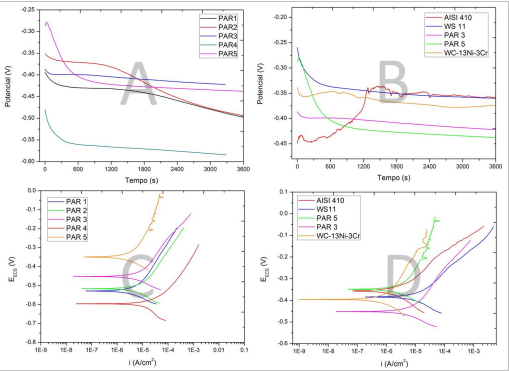
\includegraphics[width=1\columnwidth]{method/figs/adequacao/adequacao4.png}
    \caption{(A): Potencial de Circuito Aberto, com variação de parâmetros de
    aspersão térmica dos revestimentos de WC-10Co-4Cr com granulometria do pó
    11/45; (B) Potencial de Circuito Aberto de diferentes sistemas comparando
    com o substrato Jateado; (C) Ensaio de Polarização com variação de
    parâmetros dos revestimentos de WC-10Co-4Cr com granulometria do pó 11/45;
    (D) Ensaio de polarização dos diferentes sistemas comparando com o
    substrato jateado.}
    \label{fig:adequacao4}
\end{figure}

Para as curvas de OCP apresentadas na Fig.~\ref{fig:adequacao4} (B), foi
selecionado os dois revestimentos com menores porosidades nas medições
anteriores assim como o substrato, o WS 11 o qual foi utilizado pó com
granulometria diferente e o WCNi.

Conforme já comentado, os sistemas revestidos sofreram redução ao longo do tempo
pela provável modificação da solução no interior dos poros, ao contrário do
comportamento do substrato, que por ser maciço, não apresenta poros. Neste caso
observa-se um aumento do potencial de corrosão com o tempo, indicando redução no
processo corrosivo, possivelmente devido ao espessamento do filme protetor do
óxido de cromo.

Na Fig.~\ref{fig:adequacao4} (C), são apresentados os ensaios de polarização
eletroquímica da variação de alguns parâmetros operacionais. Nota-se que os
revestimentos com menores porosidades apresentam potencial de circuito aberto
(quando a curva tende a zero) mais elevado (menos negativos) indicando menor
taxa de corrosão. Além disso, à medida que a porosidade é reduzida, as curvas de
polarização tendem a se deslocar a esquerda, no sentido das menores correntes,
resultando em menores taxas de corrosão.

Na Fig.~\ref{fig:adequacao4} (D), são apresentadas as curvas de polarização dos
sistemas que tiveram menores porosidades e melhores desempenhos na
Fig.~\ref{fig:adequacao4} (C), o substrato de aço inoxidável AISI 410 jateado, a
amostra WS 11 utilizando um pó com granulometria de 15/45 e a amostra WCNi com
matriz de níquel. Analisando a Fig.~\ref{fig:adequacao4} (D), pode-se dizer
preliminarmente que os sistemas que apresentaram melhor desempenho frente a
corrosão, protegendo efetivamente o substrato, são os sistemas 5 e o WCNi. Esse
resultado é fruto de apenas uma técnica, necessitando de confirmação com outros
tipos de ensaios que considerem tempos mais longos de exposição das amostras ao
meio. Como, por exemplo, ensaio de imersão ou impedância eletroquímica.

Pode-se concluir que os teores de porosidade crescentes pioram o desempenho da
camada em proteger o substrato contra corrosão. Entre as camadas estudadas, as
que apresentaram efetiva proteção ao substrato foram os sistemas 5 e WCNi. A
presença de níquel no revestimento demonstra ser promissor em relação à proteção
do substrato à corrosão.